% !TEX root = task-3-2.tex
% Editable task bank. Append new BankTask blocks at the end of the document.
\documentclass[12pt,a4paper]{article}
\usepackage{physics-textbook}
\usepackage{graphicx,needspace}
\usetikzlibrary{decorations.pathmorphing}
\newif\ifShowSolutions
\ifdefined\TutorEdition
  \ShowSolutionstrue
\else
  \ShowSolutionsfalse % Change to \ShowSolutionstrue to display solutions.
\fi
\newcounter{banktask}
\newsavebox{\BankTaskBox}
\newcommand{\BankTaskContent}[3]{%
  \noindent\textbf{\thebanktask.}\quad #2\par
  \ifShowSolutions
    \Needspace{50mm}% Keep the solution heading with its opening text or diagram.
    #3\par
    \ifdefined\TutorEdition
      \ifcsname TutorSource#1\endcsname
        \nopagebreak\smallskip{\small\csname TutorSource#1\endcsname\par}%
      \fi
    \fi
  \fi
}
\newcommand{\BankTask}[3]{%
  \refstepcounter{banktask}\par\medskip
  \sbox{\BankTaskBox}{\begin{minipage}{\linewidth}%
    \BankTaskContent{#1}{#2}{#3}\end{minipage}}%
  \ifdim\dimexpr\ht\BankTaskBox+\dp\BankTaskBox\relax>\dimexpr\textheight-20mm\relax
    \Needspace{35mm}\BankTaskContent{#1}{#2}{#3}%
  \else
    \Needspace{\dimexpr\ht\BankTaskBox+\dp\BankTaskBox\relax}%
    \noindent\usebox{\BankTaskBox}\par
  \fi
  \medskip
}
\begin{document}
\BookSubsection{3.2}{Закон Кулона и суперпозиция сил}


% Source sdamgia-8008: https://phys-ege.sdamgia.ru/problem?id=8008
\BankTask{sdamgia-8008}{
С какой силой взаимодействуют в вакууме два маленьких заряженных шарика, находящихся на расстоянии $4 \,\text{м}$ друг от друга? Заряд каждого шарика $8 \cdot 10^{-8} \,\text{Кл}$. (В микроньютонах.)\par
}{
\smallskip\noindent\textbf{Решение}\par
Точечные заряды взаимодействую с силой $F=k \frac{ q_{1}q_{2}}{ r ^2 } =9 \cdot 10 ^{9} \cdot \frac{ 8 \cdot 10 ^{ - 8 } \cdot 8 \cdot 10 ^{ - 8 } }{ 4 ^2 } =3{,}6 \cdot 10 ^{ - 6 } \,\text{Н}=3{,}6\,\text{мкН}.$\par
Ответ: $3{,}6$.\par
}

% Source sdamgia-28084: https://phys-ege.sdamgia.ru/problem?id=28084
\BankTask{sdamgia-28084}{
Два одинаковых положительных точечных заряда $q=1 \cdot 10 ^{ - 8 } \,\text{Кл}$ расположены в вакууме и отталкиваются друг от друга с силами $40 \,\text{мкН}$. На каком расстоянии друг от друга находятся эти заряды? (В метрах.)\par
}{
\smallskip\noindent\textbf{Решение}\par
Из закона Кулона $F= \frac{ kq ^2 }{ r ^2 }$ следует, что расстояние между зарядами $r=q\sqrt{\frac{k}{F}}=1\cdot10^{-8}\sqrt{\frac{9\cdot10^9}{4\cdot10^{-5}}}=0{,}15\,\text{м}.$\par
Ответ: $0{,}15$.\par
}

% Source sdamgia-1331: https://phys-ege.sdamgia.ru/problem?id=1331
\BankTask{sdamgia-1331}{
Между двумя точечными заряженными телами сила электрического взаимодействия равна $12 \,\text{мН}$. Если заряд одного тела увеличить в $3$ раза, а заряд другого тела уменьшить в $4$ раза и расстояние между телами уменьшить в $2$ раза, то какова будет сила взаимодействия между телами? (В мН.)\par
}{
\smallskip\noindent\textbf{Решение}\par
Согласно закону Кулона, сила взаимодействия электрических зарядов прямо пропорциональна произведению величин зарядов и обратно пропорциональна квадрату расстояния между ними: $F=\frac{kq_1q_2}{r^2}.$ Таким образом, увеличение заряда одного из тел в $3$ раза, уменьшение заряда второго тела в $4$ раза и уменьшение расстояния между телами в $2$ раза приведет к увеличению силы взаимодействия в $\frac{ 3 \cdot 1/4}{ ( 1/2 ) ^2 } =3$ раза. Она станет равной $3 \cdot 12\,\text{мН}=36\,\text{мН}.$\par
Ответ: $36$.\par
}

% Source sdamgia-20888: https://phys-ege.sdamgia.ru/problem?id=20888
\BankTask{sdamgia-20888}{
Заряды $10$ и $16 \,\text{нКл}$ расположены на расстоянии $7 \,\text{мм}$ друг от друга. Какая сила будет действовать на заряд $2 \,\text{нКл}$, помещенный в точку, удаленную на $3 \,\text{мм}$ от меньшего заряда и на $4 \,\text{мм}$ от большего? (В мН.)\par
}{
\smallskip\noindent\textbf{Решение}\par

\begin{center}\begin{tikzpicture}[book diagram,>=stealth]
\draw(0,0)--(4,0);\foreach\x in{0,1.7,4}\draw[fill=white](\x,0)circle(.12);\node[left]at(0,0){$1$};\node[right]at(4,0){$2$};\draw[->,thick](1.7,0)--(.7,0)node[above]{$\vec F_2$};\draw[->,thick](1.7,0)--(2.9,0)node[above]{$\vec F_1$};\draw[<->](0,.65)--(4,.65)node[midway,above]{$7\,\text{мм}$};\draw[<->](0,-.65)--(1.7,-.65)node[midway,below]{$r_1=3\,\text{мм}$};\draw[<->](1.7,-.65)--(4,-.65)node[midway,below]{$r_2=4\,\text{мм}$};
\end{tikzpicture}\end{center}
\par
Все заряды будут находиться на одной линии, так как $3$ + $4=7$.\par
Искомая сила определяется выражением $F=F_{1} - F_{2}.$\par
Из закона Кулона:\par
\[F=k \frac{ |q_{1}| \cdot |q_{2}|}{ r ^2 } ;\]
\[F=k \frac{ |q_{1}| \cdot |q_{3}|}{ r_{1} ^2 } - k \frac{ |q_{2}| \cdot |q_{3}|}{ r_{2} ^2 } =k|q_{3}| ( \frac{ |q_{1}|}{ r_{1} ^2 } - \frac{ |q_{2}|}{ r_{2} ^2 } ) ;\]
\[F=9 \cdot 10 ^{9} \,\text{Н} \cdot \,\text{м} ^2 /\,\text{Кл} ^2 \cdot 2 \cdot 10 ^{ - 9 } \,\text{Кл} ( \frac{ 10 \cdot 10 ^{ - 9 } \,\text{Кл}}{ ( 3 \cdot 10 ^{ - 3 } \,\text{м} ) ^2 } - \frac{ 16 \cdot 10 ^{ - 9 } \,\text{Кл}}{ ( 4 \cdot 10 ^{ - 3 } \,\text{м} ) ^2 } ) =2\,\text{мН}.\]
Ответ: $2$.\par
}

% Source sdamgia-6823: https://phys-ege.sdamgia.ru/problem?id=6823
\BankTask{sdamgia-6823}{
Два точечных заряда — отрицательный, равный по модулю $3 \,\text{мкКл}$, и положительный, равный по модулю $4 \,\text{мкКл}$, расположены на расстоянии $1 \,\text{м}$ друг от друга. На расстоянии $1$ метр от каждого из этих зарядов помещают положительный заряд $Q$, модуль которого равен $2 \,\text{мкКл}$. Определите модуль силы, действующей на заряд $Q$ со стороны двух других зарядов. (В мН и округлите до целого числа.)\par
}{
\smallskip\noindent\textbf{Решение}\par

\begin{center}\begin{tikzpicture}[book diagram,>=stealth]
\coordinate(A)at(-1.5,2.6);\coordinate(B)at(1.5,2.6);\coordinate(Q)at(0,0);\draw(A)--(B)--(Q)--cycle;\fill(A)circle(1.5pt)node[above]{$-Q_1$};\fill(B)circle(1.5pt)node[above]{$+Q_2$};\fill(Q)circle(1.5pt)node[right]{$+Q$};\draw[->,thick](Q)--(-.6,1.04)node[left]{$\vec F_1$};\draw[->,thick](Q)--(-.8,-1.39)node[below]{$\vec F_2$};\draw(-.6,1.04)--(-1.4,-.35)--(-.8,-1.39);\draw[->,thick](Q)--(-1.4,-.35)node[left]{$\vec F$};
\end{tikzpicture}\end{center}
\par
Пусть $Q_{1}, Q_{2}$ — соответственно первый и второй заряды, изобразим силы, действующие на заряд $Q$ и найдем их равнодействующую (см. рис.). Заметим, что заряды лежат в вершинах равностороннего треугольника, поэтому угол между силами $\vec{F}_{1}$ и $\vec{F}_{2}$ равен $120$°. Рассмотрим треугольник $QF_{1}F,$ в нем $\angle QF_{1}F=60 ^\circ.$ Найдем модуль равнодействующей силы, используя теорему косинусов для этого треугольника:\par
\[\begin{aligned}F&=\sqrt{F_1^2+F_2^2-2F_1F_2\cos60^\circ}\\&=\sqrt{\left(k\frac{Q_1Q}{r_1^2}\right)^2+\left(k\frac{Q_2Q}{r_2^2}\right)^2-2k\frac{Q_1Q}{r_1^2}\cdot k\frac{Q_2Q}{r_2^2}\cdot\frac12}.\end{aligned}\]
По условию задачи $r_{1}=r_{2},$ поэтому:\par
\[F=k\frac{Q}{r^2}\sqrt{Q_1^2+Q_2^2-2\cdot\frac12Q_1Q_2}=\]
\[\begin{aligned}&=9\cdot10^9\frac{\text{Н}\cdot\text{м}^2}{\text{Кл}^2}\cdot\frac{2\cdot10^{-6}\,\text{Кл}}{(1\,\text{м})^2}\sqrt{\left(9+16-2\cdot\frac12\cdot3\cdot4\right)\cdot10^{-12}\,\text{Кл}^2}\\&\approx65\cdot10^{-3}\,\text{Н}=65\,\text{мН}.\end{aligned}\]
Ответ: $65$.\par
}

% Source sdamgia-7859: https://phys-ege.sdamgia.ru/problem?id=7859
\BankTask{sdamgia-7859}{
В трех вершинах квадрата размещены точечные заряды: $-q,$ +$q$, $- q$ ($q>0$) (см. рис.). Куда направлена кулоновская сила, действующая со стороны этих зарядов на точечный заряд $+2q$, находящийся в центре квадрата?\par

\begin{center}\begin{tikzpicture}[book diagram,>=stealth]
\draw(0,0)rectangle(2,2);\fill(0,0)circle(1.5pt)node[below left]{$+q$};\fill(0,2)circle(1.5pt)node[above left]{$-q$};\fill(2,0)circle(1.5pt)node[below right]{$-q$};\fill(1,1)circle(1.5pt)node[below]{$+2q$};
\end{tikzpicture}\end{center}
\par
\begin{center}\begin{tabular}{cc}1) $\rightarrow$ & 2) $\swarrow$\\3) $\nearrow$ & 4) $\nwarrow$\end{tabular}\end{center}\par
}{
\smallskip\noindent\textbf{Решение}\par
Силы притяжения со стороны отрицательных зарядов уравновешивают друг друга, поэтому суммарная сила трех зарядов совпадает с силой со стороны положительного заряда, который отталкивает центральный заряд по прямой их соединяющей, то есть вправо вверх.\par
Правильный ответ указан под номером $3$.\par
}

% Source sdamgia-39257: https://phys-ege.sdamgia.ru/problem?id=39257
\BankTask{sdamgia-39257}{
Две маленькие бусинки, закреплённые в точках А и В, несут на себе заряды $-3q$ и $+1{,}5q>0$ соответственно (см. рис.).\par
$1$) Если бусинки соединить незаряженной стеклянной палочкой, их заряды станут равными.\par
$2$) Если бусинки соединить тонкой медной проволокой, то они будут притягивать друг друга.\par
$3$) Модуль силы Кулона, действующей на бусинку В, равен модулю силы Кулона, действующей на бусинку А.\par
$4$) На бусинку А со стороны бусинки В действует сила Кулона, направленная горизонтально вправо.\par
$5$) Напряжённость результирующего электростатического поля в точке С направлена горизонтально вправо.\par

\begin{center}\begin{tikzpicture}[book diagram,>=stealth]
\draw(0,0)--(4,0);\fill(0,0)circle(2pt)node[below]{$A$}node[above]{$-3q$};\fill(2,0)circle(2pt)node[below]{$C$};\fill(4,0)circle(2pt)node[below]{$B$}node[above]{$+1{,}5q$};
\end{tikzpicture}\end{center}
\par
}{
\smallskip\noindent\textbf{Решение}\par
$1$) Неверно. Стекло является диэлектриком, поэтому при соединении бусинок стеклянной палочкой их заряды не изменятся.\par
$2$) Неверно. Медь относится к проводникам, поэтому при соединении бусинок медной проволокой их заряды станут равными по модулю и по закону сохранения заряда\par
\[q= \frac{ q_{1} + q_{2}}{ 2 } = \frac{ - 3q + 1{,}5q}{ 2 } = - 0{,}75q.\]
Такие одноименно заряженные бусинки будут отталкиваться.\par
$3$) Верно. По третьему закону Ньютона силы взаимодействия зарядов равны по модулю.\par
$4$) Верно. Заряды бусинок разноименные, поэтому они притягиваются. Следовательно, на бусинку А со стороны бусинки В действует сила Кулона, направленная горизонтально вправо.\par
$5$) Неверно. Вектор напряженности $\vec{E}_{A}$ поля, созданного бусинкой А, направлен влево. Вектор напряженности $\vec{E}_{\text{В}}$ поля, созданного бусинкой В, направлен влево. По принципу суперпозиции полей результирующий вектор $\vec{E}=\vec{E}_{A} + \vec{E}_{B}$ направлен влево.\par
Ответ: $34$.\par
}

% Source sdamgia-3659: https://phys-ege.sdamgia.ru/problem?id=3659
\BankTask{sdamgia-3659}{
Два точечных заряда $q_{1}$ и $q_{2},$ находящиеся на расстоянии $r=1 \,\text{м}$ друг от друга, притягиваются с силой $F=1\,\text{Н}.$ Сумма зарядов равна $Q=2 \,\text{мкКл}.$ Чему равны модули этих зарядов?\par
}{
\smallskip\noindent\textbf{Решение}\par
Поскольку заряды притягиваются, знаки $q_{1}$ и $q_{2}$ различны. Будем считать, что $q_{1} > 0,$ $a$ $q_{2} < 0.$ Из условия следует, что $q_{1} - |q_{2}|=Q.$\par
Согласно закону Кулона $F=k \frac{ q_{1}|q_{2}|}{ r ^2 } .$\par
Из написанных уравнений получаем:\par
$q_{1}=Q + |q_{2}|,$ $\frac{ Fr ^2 }{ k } =|q_{2}| \cdot ( Q + |q_{2}| ) .$\par
Таким образом, $|q_{2}| ^2 + Q|q_{2}| - \frac{ Fr ^2 }{ k } =0.$\par
Отсюда:\par
\[|q_2|=-\frac Q2\pm\sqrt{\frac{Q^2}{4}+\frac{Fr^2}{k}},\]
причем перед корнем следует выбрать знак « + », так как $|q_{2}| > 0.$ Окончательно имеем:\par
$|q_2|=-\frac Q2+\sqrt{\frac{Q^2}{4}+\frac{Fr^2}{k}},$ $q_1=Q+|q_2|=\frac Q2+\sqrt{\frac{Q^2}{4}+\frac{Fr^2}{k}}.$\par
Подставляя числовые данные, получаем:\par
\[|q_1|=\frac{2\cdot10^{-6}}2+\sqrt{\frac{4\cdot10^{-12}}4+\frac{1\cdot1}{9\cdot10^9}}\approx11{,}6\,\text{мкКл},\]
\[|q_2|=-\frac{2\cdot10^{-6}}2+\sqrt{\frac{4\cdot10^{-12}}4+\frac{1\cdot1}{9\cdot10^9}}\approx9{,}6\,\text{мкКл}.\]
Ответ: $|q_{1}|\approx 11{,}6 \,\text{мкКл},$ $|q_{2}|\approx 9{,}6 \,\text{мкКл}.$\par
Примечание. Систему уравнений легко решить, если применить теорему Виета:\par
\[q_{1} + q_{2}=Q\]
\[q_1q_2=-\frac{Fr^2}{k}.\]
По теореме Виета величины $q_{1}$ и $q_{2}$ являются корнями квадратного уравнения, у которого $a=1;$ $b= - Q;$ $c= - \frac{ Fr ^2 }{ k } .$\par
}

% Source sdamgia-3063: https://phys-ege.sdamgia.ru/problem?id=3063
\BankTask{sdamgia-3063}{
При облучении металлической пластинки быстрыми $\alpha$-частицами небольшая часть этих частиц в результате упругого взаимодействия с ядрами атомов меняет направление скорости на противоположное (аналог опыта Резерфорда). Найдите заряд ядра, если минимальное расстояние, на которое сближались ядро и частица, составило $5 \cdot 10 ^{ - 13 } \,\text{см}.$ Масса и скорость $\alpha$-частиц на большом расстоянии от пластины составляют соответственно $7 \cdot 10 ^{ - 27 } \,\text{кг}$ и $26 \cdot 10 ^3 \,\text{км}/\,\text{с}.$ (Частицу считать точечной, а ядро — точечным и неподвижным. Релятивистским эффектом пренебречь. Потенциальная энергия кулоновского взаимодействия ядра и $\alpha$-частицы $E_{\text{пот}}=k \frac{ q_ \alpha q_{\text{ядра}}}{ r } ,$ где $r$ — расстояние между ядром и $\alpha$-частицей.)\par
}{
\smallskip\noindent\textbf{Решение}\par
Точечные заряды при взаимодействии обладают энергией $W=k \frac{ q_ \alpha q_{\text{ядра}}}{ r } ,$ где $q_ \alpha =2e$ - заряд $\alpha$-частицы.\par
Изменение кинетической энергии альфа-частицы при сближении с ядром равно $E_{\text{к}}= \frac{ m v ^2 }{ 2 } .$\par
Изменение кинетической энергии равно энергии взаимодействия зарядов на минимальном расстоянии между $\alpha$-частицей и ядром: $W=E_{\text{к}}.$\par
Выполняем соответствующие математические преобразования, получен ответ в общем виде:\par
\[q_{\text{ядра}}= \frac{ m v ^2 r}{ 2kq_ \alpha } = \frac{ m v ^2 r}{ 4k|e| } .\]
Числовой ответ: $q_{\text{ядра}}= \frac{ 7 \cdot 10 ^{ - 27 } \cdot ( 26 \cdot 10 ^{ 6 } ) ^2 \cdot 5 \cdot 10 ^{ - 15 } }{ 4 \cdot 9 \cdot 10 ^{9} \cdot 1{,}6 \cdot 10 ^{ - 19 } } \approx 4 \cdot 10 ^{ - 18 } \,\text{Кл}.$\par
Ответ: $q_{\text{ядра}}=4 \cdot 10 ^{ - 18 } \,\text{Кл}.$\par
}

% Source sdamgia-31902: https://phys-ege.sdamgia.ru/problem?id=31902
\BankTask{sdamgia-31902}{
К крючку на потолке подвесили на легких диэлектрических нитях длиной $l=1 \,\text{м}$ два одинаковых маленьких шарика массой $m=10 \,\text{г}$ каждый и сообщили им одинаковые заряды $q$. После этого шарики оттолкнулись друг от друга, и когда колебания затухли, оказалось, что в положении равновесия угол между нитями равен $2 \alpha = 60 ^\circ .$ Найдите величину и знак зарядов $q$.\par
}{
\smallskip\noindent\textbf{Решение}\par

\begin{center}\begin{tikzpicture}[book diagram,>=stealth]
\draw(-.3,3)--(.3,3);\foreach\x in{-.3,-.15,0,.15,.3}\draw(\x,3)--++(.12,.12);\draw(0,3)--(-1.5,.4)(0,3)--(1.5,.4);\node[left]at(-1.15,2.1){$l$};\node[right]at(1.15,2.1){$l$};\draw(0,3)--(0,.4);\draw(-1.5,.4)--(1.5,.4)node[midway,below]{$r$};\draw(0,2.45)arc(-90:-120:.55);\draw(0,2.45)arc(-90:-60:.55);\node at(-.2,2.25){$\alpha$};\node at(.2,2.25){$\alpha$};\foreach\x/\sign in{-1.5/-1,1.5/1}{\draw[fill=white](\x,.4)circle(.09);\draw[->,thick](\x,.4)--++(\sign*.7,0)node[above]{$\vec F$};\draw[->,thick](\x,.4)--++(0,-.8)node[below]{$m\vec g$};\draw[->,thick](\x,.4)--++(-\sign*.55,.95)node[above]{$\vec T$};}\draw[thin](-.95,1.35)--(-.95,.4)--(-1.5,-.4)(.95,1.35)--(.95,.4)--(1.5,-.4);\draw(-.95,1.10)arc(-90:-120:.25);\draw(.95,1.10)arc(-90:-60:.25);\draw[->](.35,1.65)--(.35,.95)node[left,midway]{$\vec g$};
\end{tikzpicture}\end{center}
1. Изобразим систему в положении равновесия (см. рис.).\par
$2$. На каждый из зарядов действует вертикальная сила тяжести mg, горизонтальная (в силу симметрии системы) кулоновская сила отталкивания $F$ и направленная вдоль нити сила ее натяжения $T$.\par
$3$. В равновесии векторная сумма этих трех сил равна нулю, как и суммы проекций сил на вертикальное и горизонтальное направления: $T \cos \alpha =mg,$ $T \sin \alpha =F.$ Отсюда:\par
$T= \frac{ mg}{ \cos \alpha } ,$ а $F= mg \tan \alpha .$\par
$4$. Согласно закону Кулона $F= \frac{ kq ^2 }{ r ^2 } ,$ где расстояние между зарядами $r=2l \sin \alpha .$\par
$5$. Подставляя записанные выражения в уравнение $F= mg \tan \alpha ,$ получаем:\par
\[\frac{ kq ^2 }{ ( 4l ^2 \sin ^2 \alpha ) } =mg \tan \alpha ,\]
откуда:\par
$q ^2 = \frac{ 4l ^2 mg \sin ^2 \alpha \tan \alpha }{ k }$ и $q=\pm2l\sin\alpha\left(\frac{mg\tan\alpha}{k}\right)^{1/2}.$\par
$6$. По условию $\alpha =30 ^\circ,$ так что $\sin \alpha = \frac{ 1}{ 2 }$ или $\tan\alpha=\left(\frac13\right)^{1/2}.$ Подставляя численные данные из условия задачи в системе СИ, получаем:\par
\[q=\pm2\cdot1\cdot0{,}5\left[\frac{10^{-2}\cdot10\cdot1}{3^{1/2}\cdot9\cdot10^9}\right]^{1/2}\approx\pm2{,}533\cdot10^{-6}\,\text{Кл}=\pm2{,}533\,\text{мкКл}.\]
Ответ: ±$2{,}533 \,\text{мкКл}$.\par
}


% Source 3BB12E: https://ege.fipi.ru/bank/questions.php?search=1&proj=BA1F39653304A5B041B656915DC36B38&qid=3BB12E
\BankTask{3BB12E}{
Одинаковые отрицательные точечные заряды, модуль которых $|q|=2\cdot10^{-8}\,\text{Кл}$, расположены в вакууме на расстоянии $3\,\text{м}$ друг от друга. Определите модуль сил взаимодействия этих зарядов друг с другом.

Ответ выразите в $\text{мкН}$. (в $\text{мкН}$).
}{
\smallskip\noindent\textbf{Решение от GPT}\par
По закону Кулона при $k_{\text{К}}=9\cdot10^9\,\text{Н}\cdot\text{м}^2/\text{Кл}^2$:
\[
F=k_{\text{К}}\frac{|q|^2}{r^2}=9\cdot10^9\frac{(2\cdot10^{-8})^2}{3^2}=4\cdot10^{-7}\,\text{Н}=0{,}4\,\text{мкН}.
\]
Ответ: $0{,}4\,\text{мкН}$.
}

% Source D48CE0: https://ege.fipi.ru/bank/questions.php?search=1&proj=BA1F39653304A5B041B656915DC36B38&qid=D48CE0
\BankTask{D48CE0}{
Два неподвижных заряженных шарика, находящихся в вакууме на расстоянии $0{,}3\,\text{м}$ друг от друга, притягиваются друг к другу с силой $8\cdot10^{-9}\,\text{Н}$. Чему равен модуль заряда второго шарика, если заряд первого составляет $2\cdot10^{-10}\,\text{Кл}$? Ответ выразите в нанокулонах ($\text{нКл}$). (в $\text{нКл}$).
}{
\smallskip\noindent\textbf{Решение от GPT}\par
По закону Кулона при $k_{\text{К}}=9\cdot10^9\,\text{Н}\cdot\text{м}^2/\text{Кл}^2$:
\[
|q_2|=\frac{Fr^2}{k_{\text{К}}|q_1|}=\frac{8\cdot10^{-9}\cdot(0{,}3)^2}{9\cdot10^9\cdot2\cdot10^{-10}}=4\cdot10^{-10}\,\text{Кл}=0{,}4\,\text{нКл}.
\]
Ответ: $0{,}4\,\text{нКл}$.
}

% Source 8FC4FE: https://ege.fipi.ru/bank/questions.php?search=1&proj=BA1F39653304A5B041B656915DC36B38&qid=8FC4FE
\BankTask{8FC4FE}{
Два неподвижных точечных заряда действуют друг на друга с силами, модуль которых равен $F$. Во сколько раз увеличится модуль этих сил, если оба заряда увеличить в $3$ раза, а расстояние между ними увеличить в $2$ раза?
}{
\smallskip\noindent\textbf{Решение от GPT}\par
По закону Кулона $F\propto |q_1q_2|/r^2$, поэтому
\[
\frac{F'}{F}=\frac{3\cdot3}{2^2}=\frac94=2{,}25.
\]
Ответ: в $2{,}25$ раза.
}

% Source 11272F: https://ege.fipi.ru/bank/questions.php?search=1&proj=BA1F39653304A5B041B656915DC36B38&qid=11272F
\BankTask{11272F}{
Во сколько раз уменьшится модуль сил взаимодействия двух небольших металлических шариков одинакового диаметра, имеющих заряды \(q_1=+7\,\text{нКл}\) и \(q_2=-3\,\text{нКл}\), если шарики привести в соприкосновение и раздвинуть на прежнее расстояние?
}{
\smallskip\noindent\textbf{Решение от GPT}\par
После соприкосновения заряды одинаковых шариков равны: \(q'=(q_1+q_2)/2=2\,\text{нКл}\). По закону Кулона при прежнем расстоянии
\[
\frac{F}{F'}=\frac{|q_1q_2|}{(q')^2}=\frac{7\cdot3}{2^2}=5{,}25.
\]
Ответ: уменьшится в \(5{,}25\) раза.
}

% Source 2583B9: https://ege.fipi.ru/bank/questions.php?search=1&proj=BA1F39653304A5B041B656915DC36B38&qid=2583B9
\BankTask{2583B9}{
\begin{center}
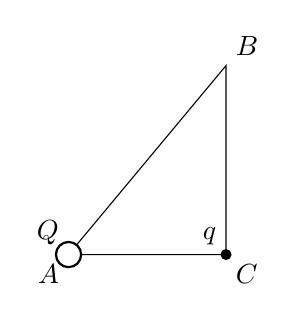
\begin{tikzpicture}[>=stealth,scale=1]
\coordinate (A) at (0,0);
\coordinate (C) at (2,0);
\coordinate (B) at (2,2.4);
\draw (A)--(B)--(C)--cycle;
\fill[white] (A) circle (0.16);
\draw[thick] (A) circle (0.16);
\fill (C) circle (0.07);
\node[below left] at (A) {$A$};
\node[above left] at (A) {$Q$};
\node[below right] at (C) {$C$};
\node[above left] at (C) {$q$};
\node[above right] at (B) {$B$};
\end{tikzpicture}
\end{center}
В треугольнике \(ABC\) угол \(C\) прямой, \(BC=0{,}8\,\text{м}\). В вершине \(A\) находится точечный заряд \(Q\). Он действует с силой \(2{,}5\cdot10^{-8}\,\text{Н}\) на точечный заряд \(q\), помещённый в вершину \(C\). Если заряд \(q\) перенести в вершину \(B\), то заряды будут взаимодействовать с силой \(9{,}0\cdot10^{-9}\,\text{Н}\). Найдите \(AC\). (в $\text{м}$).
}{
\smallskip\noindent\textbf{Решение от GPT}\par
По закону Кулона \(F_C/F_B=AB^2/AC^2=25/9\). По теореме Пифагора \(AB^2=AC^2+BC^2\), поэтому
\[
\frac{25}{9}=1+\frac{0{,}8^2}{AC^2},\qquad
AC=\sqrt{\frac{0{,}64\cdot9}{16}}=0{,}6\,\text{м}.
\]
Ответ: \(0{,}6\,\text{м}\).
}

% Source 7D9e2D: https://ege.fipi.ru/bank/questions.php?search=1&proj=BA1F39653304A5B041B656915DC36B38&qid=7D9e2D
\BankTask{7D9e2D}{
Две маленькие закреплённые проводящие бусинки, расположенные в точках $A$ и $B$, несут на себе заряды $+3q>0$ и $-1{,}5q<0$ соответственно (см. рисунок). Точка $C$ находится посередине между бусинками $A$ и $B$.
\begin{enumerate}
\item На бусинку $B$ со стороны бусинки $A$ действует сила Кулона, направленная горизонтально вправо.
\item Напряжённость результирующего электростатического поля в точке $C$ направлена горизонтально влево.
\item Модули сил Кулона, действующих на бусинки, одинаковы.
\item Если бусинки соединить тонкой стальной проволокой, они начнут отталкиваться друг от друга.
\item Если бусинки соединить незаряженной стеклянной палочкой, их заряды станут одинаковыми.
\end{enumerate}
\begin{center}
\begin{tikzpicture}[book diagram]
\draw[densely dashed] (0,0)--(4,0);
\fill (0,0) circle (2pt) node[above=7pt] {$+3q$} node[below=5pt] {$A$};
\fill (2,0) circle (2pt) node[below=5pt] {$C$};
\fill (4,0) circle (2pt) node[above=7pt] {$-1{,}5q$} node[below=5pt] {$B$};
\end{tikzpicture}
\end{center}
}{
\smallskip\noindent\textbf{Решение от GPT}\par
1) Неверно: разноимённые заряды притягиваются, поэтому сила на бусинку $B$ направлена влево. 2) Неверно: в точке $C$ оба поля направлены вправо — от положительного заряда к отрицательному. 3) Верно по третьему закону Ньютона: $F_{AB}=F_{BA}$. 4) Верно: при соединении проводником суммарный положительный заряд $3q-1{,}5q=1{,}5q$ перераспределится, и бусинки будут отталкиваться. 5) Неверно: стекло — диэлектрик и не обеспечивает перетекания зарядов между бусинками. Ответ: $3,\ 4$.
}

\end{document}
